\documentclass{article}
% NeurIPS 2026 style; [preprint] shows author names. The footer is replaced below.
\usepackage[preprint]{neurips_2026}
\makeatletter
\renewcommand{\@noticestring}{ESE 5420 Final Project, University of Pennsylvania. Early paper draft, November 2026.}
\makeatother

\usepackage[utf8]{inputenc}
\usepackage[T1]{fontenc}
\usepackage{hyperref}
\hypersetup{colorlinks=true,linkcolor=black,citecolor=black,urlcolor=blue}
\usepackage{url}
\usepackage{booktabs}
\usepackage{amsmath,amsfonts}
\usepackage{microtype}
\usepackage{xcolor}
\usepackage{graphicx}
\usepackage{enumitem}
\setlist{nosep}

\newcommand{\bp}{\,\mathrm{bp}}
\newcommand{\RMSE}{\operatorname{RMSE}}

\title{Can Lagged Yield Changes Beat a Random Walk?\\
One-Day Forecasts of the 10-Year U.S.\ Treasury Yield}

\author{%
  Jonah Engelmann \qquad Leo Gordon \qquad Malcolm Siljehag Alencar \\
  \textmd{University of Pennsylvania, ESE 5420}
}

\begin{document}
\maketitle

\begin{abstract}
Can a model fitted to recent daily changes in the 10-year U.S.\ Treasury yield forecast the next day's change more accurately than a random walk, which predicts no change? We study this with public Treasury par-yield data for 2020--2023. Our course baseline is ordinary least squares (OLS) on the last $p$ daily changes. We tune $p$ by expanding-window validation over the eight quarters of 2021--2022 and evaluate once on 2023, scoring root mean squared error (RMSE) in basis points (bp). On 2023 the baseline's RMSE is 7.486\,bp, against 7.461\,bp for the zero-change forecast: a difference of 0.025\,bp with a 95\% paired block-bootstrap interval of $[-0.018, 0.066]$\,bp. The interval contains zero, so in this preliminary result the baseline ties the random walk. The remaining experiments test whether that tie survives more information (lagged changes at other maturities, yield-curve spreads and recent volatility), more flexible models ($k$-nearest neighbors, a random forest) and a fresh, untouched test period (2024--2025).
\end{abstract}

\section{Introduction}
Daily changes in long-term interest rates matter to anyone who holds or hedges bonds: a change of a few basis points in the 10-year Treasury yield moves the value of large portfolios, and the 10-year yield is a reference rate for mortgages and corporate borrowing. A forecast of tomorrow's change is only useful, however, if it beats the simplest possible forecast: that tomorrow's yield equals today's. This \emph{random walk} benchmark is famously hard to beat out of sample in financial markets. \citet{meese1983} found that standard structural models did not beat it for exchange rates at horizons of one to twelve months, and \citet{diebold2006} report that it is a demanding benchmark for yield forecasts at short horizons.

We ask a narrow, testable version of the question: \emph{do the last few daily changes of the 10-year yield predict the next one better than a forecast of zero change, by more than the sampling error of the comparison?} A finding that they do would point to short-term momentum or mean reversion. A careful null result is also informative, since it bounds how much predictive information this kind of model can extract.

We compare three forecasts on the same data and the same time-ordered validation: (i) the zero-change forecast, which the fitted models must beat; (ii) OLS on lagged changes, our course baseline; and (iii) $k$-nearest neighbors ($k$NN) on the same inputs, a flexible nonparametric comparison. Section~\ref{sec:remaining} adds ridge, the lasso and a random forest on a richer cross-maturity feature set, evaluated on a new test period. Every step learned from data, including feature scaling, is fitted inside each training window, and the test year is used once, after all tuning.

\section{Data}\label{sec:data}
\paragraph{Source.} We use the U.S.\ Department of the Treasury's \href{https://home.treasury.gov/resource-center/data-chart-center/interest-rates/daily-treasury-rate-archives/par-yield-curve-rates-2020-2023.csv}{Daily Treasury Par Yield Curve Rates archive for 2020--2023} \citep{treasury2020}. These are public U.S.\ government data, which are not subject to U.S.\ copyright, so figures derived from them can be redistributed.

\paragraph{Size and shape.} The file has 1,001 rows (trading days from 2 January 2020 to 29 December 2023) and 14 columns: the date and par yields at 13 maturities from 1 month to 30 years, in percent. The only missing values are in the 4-month column, which Treasury introduced in October 2022 (701 blank rows). There are no duplicate dates, and the 10-year yield, the only column used so far, has no missing values. We sort by date and difference consecutive trading days without filling non-trading days.

\paragraph{Target and inputs.} Let $r_t$ be the 10-year par yield on trading day $t$. The target and the inputs of a lag-$p$ model are
\begin{equation}
  y_t = 100\,(r_t - r_{t-1}) \bp, \qquad x_t^{(p)} = (y_{t-1}, \ldots, y_{t-p})^\top \in \mathbb{R}^p,
  \label{eq:features}
\end{equation}
so $x_t^{(p)}$ is known before $r_t$ is published. Yields are quoted to two decimals, so every $y_t$ is a whole number of basis points; across the four years $y_t$ takes only 46 distinct values. Table~\ref{tab:data} summarizes the data by year; the RMSE of the zero-change forecast equals the root mean square of $y_t$ and measures how volatile each year was.

\begin{table}[t]
  \caption{Observations by year and the RMSE of the zero-change forecast. The first change of 2020 has no predecessor; later years difference against the previous year's last quote.}
  \label{tab:data}
  \centering
  \begin{tabular}{lrrrl}
    \toprule
    Year & Yield obs. & Yield changes & Zero-change RMSE (bp) & Role\\
    \midrule
    2020 & 251 & 250 & 5.504 & training only\\
    2021 & 251 & 251 & 4.277 & validation quarters 1--4\\
    2022 & 249 & 249 & 7.828 & validation quarters 5--8\\
    2023 & 250 & 250 & 7.461 & held-out test\\
    \bottomrule
  \end{tabular}
\end{table}

\paragraph{Split.} The split is chronological and never shuffled. Hyperparameters are chosen on eight validation quarters, 2021\,Q1 to 2022\,Q4; each is predicted by a model trained on every observation before it, starting in January 2020 (an expanding window). After tuning, the chosen model is refitted once on 2020--2022 and scored on the 250 changes of 2023. Building lags drops the first $p+1$ days of 2020 from training, so all candidates see identical validation and test days.

\section{Methods}\label{sec:methods}
\paragraph{Zero-change forecast (reference).} $\widehat y_t^{(0)} = 0$, equivalently $\widehat r_t = r_{t-1}$: a random walk in the yield level. It has no parameters.

\paragraph{Course baseline: OLS on lagged changes.} $\widehat y_t = \widehat\beta_0 + \widehat\beta^\top x_t^{(p)}$, fitted by ordinary least squares with an intercept. The only hyperparameter is the lag length $p \in \{1,\dots,5\}$.

\paragraph{Comparison: $k$-nearest neighbors.} $\widehat y_t = \frac{1}{k}\sum_{i \in \mathcal N_k(x_t^{(p)})} y_i$, the mean target of the $k$ training days whose lagged changes are closest in Euclidean distance after standardization. The standardization is fitted on each training window only. Hyperparameters are $p \in \{1,\dots,5\}$ and $k \in \{3, 5, 10, 20, 40\}$.

\paragraph{Tuning.} The course tunes hyperparameters by $K$-fold cross-validation inside the training data. Shuffled $K$-fold would let a model train on days after the days it predicts, so we use its time-ordered analogue, expanding-window validation \citep{bergmeir2012}. The eight validation quarters play the role of the $K$ folds, and every fold is predicted from the past only. For each candidate we compute the RMSE on each quarter and select the candidate with the lowest mean of the eight quarterly RMSEs, breaking ties toward smaller $p$ and $k$. All of 2023 is excluded from this step. When forecasting 2023, the refitted model uses observed earlier 2023 changes as lags but is never refitted on them.

\section{Experimental setup}\label{sec:setup}
\paragraph{Metric.} For model $m$ evaluated on $n$ days,
\begin{equation}
  \RMSE_m = \Big(\tfrac{1}{n}\textstyle\sum_{t=1}^{n} (y_t - \widehat y_{m,t})^2\Big)^{1/2}, \qquad D_m = \RMSE_m - \RMSE_0,
  \label{eq:delta}
\end{equation}
in basis points. A negative $D_m$ means the model beats the zero-change forecast.

\paragraph{Validation error bars.} For each candidate we report the mean $\pm$ the sample standard deviation of its eight quarterly RMSEs. The standard deviation shows how much the error level moves from quarter to quarter, not the uncertainty in the difference between two models.

\paragraph{Test error bars.} Daily yield changes are serially dependent and volatility clusters, so an i.i.d.\ bootstrap of test days would understate uncertainty. We use a paired moving-block bootstrap \citep{kunsch1989} in its circular form: draw blocks of 20 consecutive test days (about one trading month) with replacement, letting a block that runs past the end of the year wrap around to its start so that every day is equally likely to be drawn, until 250 days are drawn; recompute $\RMSE_m$, $\RMSE_0$ and $D_m$ on the \emph{same} resampled days; repeat 10,000 times; and report the 2.5\% and 97.5\% percentiles of $D_m$. Pairing the two forecasts on the same days removes the shared volatility from the comparison. As a sensitivity check we repeat the bootstrap with 10- and 30-day blocks (5,000 resamples each). The intervals are conditional on the fitted model and do not include uncertainty from hyperparameter selection.

\paragraph{Reproducibility.} The models and folds are deterministic, and the bootstrap uses seed 5420. A single script produces every number in this draft from the raw CSV, and a second script fills the tables and figure from its output.

\section{Preliminary results}\label{sec:results}
\paragraph{Validation.} Table~\ref{tab:cv} lists the validation RMSE of every baseline candidate. Lag length $p=1$ has the lowest mean, so it is selected. No candidate beats the zero-change forecast on average over the eight quarters, and every difference is a small fraction of the quarter-to-quarter spread. Figure~\ref{fig:cv} shows why: the error level nearly doubles from 2021 to 2022 as rate volatility rises, while the baseline and the zero-change forecast stay almost on top of each other in every quarter.

\begin{table}[t]
  \caption{Expanding-window validation RMSE over the eight quarters of 2021--2022 (bp): mean $\pm$ sample standard deviation across quarters. The lowest mean selects the lag length. The zero-change forecast is not beaten, and all differences are far smaller than the spread across quarters.}
  \label{tab:cv}
  \centering
  \begin{tabular}{llc}
    \toprule
    Forecast & Hyperparameter & Validation RMSE (bp)\\
    \midrule
    Zero change (reference) & --- & 6.028 $\pm$ 1.993\\
    OLS (baseline) & $p=1$ & 6.052 $\pm$ 1.963\\
    OLS & $p=2$ & 6.068 $\pm$ 1.922\\
    OLS & $p=3$ & 6.079 $\pm$ 1.955\\
    OLS & $p=4$ & 6.087 $\pm$ 1.957\\
    OLS & $p=5$ & 6.113 $\pm$ 1.952\\
    \bottomrule
  \end{tabular}
\end{table}

\begin{figure}[t]
  \centering
  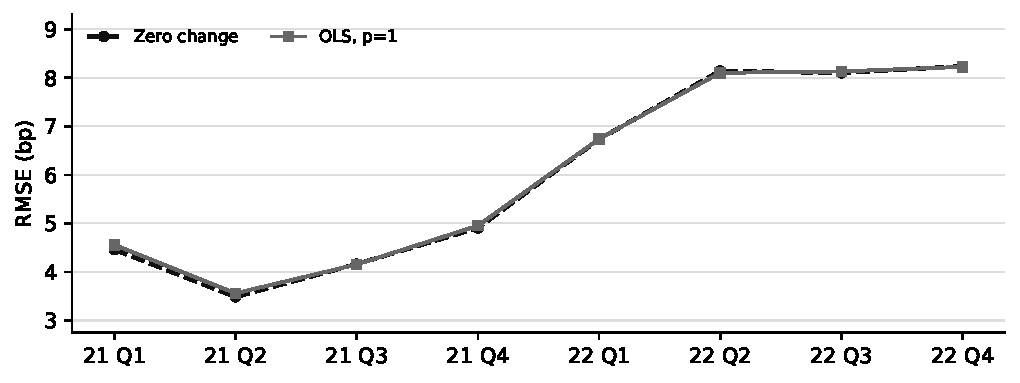
\includegraphics[width=\linewidth]{validation_rmse_draft.pdf}
  \caption{RMSE in each validation quarter for the zero-change forecast and the selected baseline (OLS, $p=1$), each fitted only on days before the quarter. The error level changes far more across quarters than between the two forecasts.}
  \label{fig:cv}
\end{figure}

\paragraph{Held-out 2023 test.} Table~\ref{tab:test} gives the single evaluation on 2023. The refitted baseline is $\widehat y_t = 0.269 + 0.033\,y_{t-1}$ (bp): the slope is close to zero, so the forecast is nearly a constant, and the model can do little more than the zero-change forecast. Its RMSE is 0.025\,bp higher, and the 95\% interval $[-0.018, 0.066]$\,bp contains zero. The two forecasts are therefore tied at this precision: the baseline neither beats nor clearly loses to the random walk. The conclusion does not depend on the block length; with 10- and 30-day blocks the intervals are $[-0.017, 0.064]$ and $[-0.014, 0.066]$\,bp.

\begin{table}[t]
  \caption{Held-out 2023 forecasts ($n=250$ days). $D$ is the model's RMSE minus the zero-change RMSE (negative favors the model). The interval is a paired circular block bootstrap (20-day blocks, 10,000 resamples). It contains zero, so the baseline ties the random walk.}
  \label{tab:test}
  \centering
  \begin{tabular}{lccc}
    \toprule
    Forecast & RMSE (bp) & $D$ (bp) & 95\% interval for $D$ (bp)\\
    \midrule
    Zero change (reference) & 7.461 & --- & ---\\
    OLS baseline ($p=1$) & 7.486 & 0.025 & $[-0.018, 0.066]$\\
    \bottomrule
  \end{tabular}
\end{table}

\paragraph{$k$NN results are withheld from this draft.} A from-scratch rerun of our code did not reproduce the $k$NN numbers exactly, although the baseline numbers reproduced to every digit. The cause is the integer-valued data noted in Section~\ref{sec:data}: with only 46 distinct daily changes, many training days lie at exactly the same distance from a query, and which of them count among the $k$ neighbors depends on the tie-breaking of the library version. The selected configuration ($p=2$, $k=40$) and the qualitative conclusion (no improvement over zero change) were the same in both runs, but the numbers differed in the second decimal. We will report $k$NN after making its tie handling deterministic (Experiment~0 below).

\section{Remaining work}\label{sec:remaining}
Because 2023 has now been inspected, it can no longer serve as an untouched test set for new models or features. Every remaining comparison therefore moves to a fresh test period, 2024--2025, which no one in the group has yet examined. Treasury publishes these years as separate files (249 and 248 trading days; the 2025 file adds a 1.5-month maturity, which we will not use). The 2023 result above stays in the paper as reported.

\subsection{Experiments to finish before Analysis Complete (30 November)}
\begin{enumerate}[leftmargin=*,label=\textbf{Exp.~\arabic*:},start=0,itemsep=3pt]
  \item \textbf{Reproducible $k$NN.} Make neighbor selection deterministic under ties (break ties by date, or average over all days tied at the $k$-th distance), pin library versions, and have a second group member rerun the whole pipeline from scratch.
  \item \textbf{New split.} Tune on twelve expanding-window quarters (2021\,Q1--2023\,Q4), refit on 2020--2023, and evaluate once on 2024--2025 ($n \approx 497$), with the same bootstrap. Report $D$ for each test year separately as well as pooled, to see whether a result holds in both.
  \item \textbf{Richer features with regularized linear models.} Add lagged daily changes of the 2-year and 30-year yields, the previous day's 2s10s and 10s30s spreads, and the standard deviation of the 10-year change over the previous 20 days (past data only). Fit ridge and the lasso (course material), with the penalty and lag length tuned in the validation quarters and standardization fitted inside each training window. This tests whether the null result is a consequence of the narrow information set.
  \item \textbf{A flexible model.} Fit a random forest (later course material) on both feature sets, tuning the leaf size and the number of features tried per split. To avoid reporting the best of many runs, we fix five seeds in advance and report the mean and spread over all five.
  \item \textbf{Wider $k$NN grid.} The selected $k=40$ is the largest value searched. Extending the grid to $k \in \{80, 160, 320\}$ shows whether $k$NN simply improves as it approaches the training-mean forecast.
\end{enumerate}

\paragraph{Key figure.} Experiments~1--4 fill a two-by-two design that separates \emph{more information} from \emph{more flexibility}: \{10-year lags only, rich features\} $\times$ \{linear (OLS, ridge, lasso), flexible ($k$NN, random forest)\}. The main figure will plot, for each model, $D$ on 2024--2025 with its 95\% block-bootstrap interval, with a vertical line at $D=0$; a model beats the random walk only if its whole interval lies to the left of that line. We will also add paired per-quarter differences to the validation results, since they measure model differences more directly than the spread of quarterly RMSEs.

\paragraph{Timeline.} Week of 16 November: Experiments 0, 1 and 4. Week of 23 November: Experiments 2 and 3, the key figure, and sensitivity checks (block length, per-year results). Analysis complete on 30 November; paper and video drafts by 4 December.

\subsection{Outline of the remaining sections}
\begin{enumerate}[leftmargin=*,itemsep=2pt]
  \item \textbf{Introduction:} add related work on random-walk benchmarks and short-horizon yield forecasting.
  \item \textbf{Data:} add the 2024--2025 files, the cross-maturity inputs and the new split.
  \item \textbf{Methods:} add ridge, the lasso and the random forest, and the deterministic $k$NN.
  \item \textbf{Experimental setup:} unchanged apart from the twelve-quarter validation and per-year test results.
  \item \textbf{Results:} validation over the twelve quarters; the 2023 result reported here; the 2024--2025 comparison (key figure); sensitivity to block length and per-year results.
  \item \textbf{Discussion and limitations:} what a tie implies, how volatility regimes drive the error level, and the limits of two test years and a single maturity.
  \item \textbf{Conclusion:} a direct answer to the question in the abstract.
  \item \textbf{Appendix:} full validation grids for every model.
\end{enumerate}

\begin{thebibliography}{9}
\bibitem[Bergmeir and Ben\'itez(2012)]{bergmeir2012}
C.~Bergmeir and J.~M. Ben\'itez. On the use of cross-validation for time series predictor evaluation. \emph{Information Sciences}, 191:192--213, 2012.

\bibitem[Diebold and Li(2006)]{diebold2006}
F.~X. Diebold and C.~Li. Forecasting the term structure of government bond yields. \emph{Journal of Econometrics}, 130(2):337--364, 2006.

\bibitem[K\"unsch(1989)]{kunsch1989}
H.~R. K\"unsch. The jackknife and the bootstrap for general stationary observations. \emph{The Annals of Statistics}, 17(3):1217--1241, 1989.

\bibitem[Meese and Rogoff(1983)]{meese1983}
R.~A. Meese and K.~Rogoff. Empirical exchange rate models of the seventies: Do they fit out of sample? \emph{Journal of International Economics}, 14(1--2):3--24, 1983.

\bibitem[{U.S. Department of the Treasury}(n.d.)]{treasury2020}
U.S.\ Department of the Treasury. Daily Treasury par yield curve rates, 2020--2023. \url{https://home.treasury.gov/resource-center/data-chart-center/interest-rates/daily-treasury-rate-archives/par-yield-curve-rates-2020-2023.csv}. Accessed November 2026.
\end{thebibliography}

\end{document}
